\documentclass[twocolumn]{article}
\usepackage[utf8]{inputenc}
\usepackage{amsmath}
\usepackage{graphicx}
\usepackage{hyperref}
\usepackage{overpic}
\usepackage{titlesec}
\usepackage{quantikz}
\usepackage{subcaption}
\usepackage{booktabs}
\usepackage{enumitem}
\usepackage[absolute,overlay]{textpos} % Required for positioning
\usepackage{lmodern}
\usepackage[a4paper,margin=1.2cm]{geometry}
\usepackage{multicol}

% Reduce space around titles
\titlespacing{\section}{0pt}{*0.5}{*0.5}
\titlespacing{\subsection}{0pt}{*0.5}{*0.5}

\title{\vspace{-1.5cm}\textbf{Research Statement}}
\author{\textbf{Uday Mathur}\\ 
        \textit{Department of Physics},\,\,
        \textit{Indian Institute of Technology (BHU), Varanasi}\\}
\date{}
\begin{document}

\twocolumn[
\maketitle

\vspace{-0.3cm}  % Adjusts space after the title

\begin{center}
    \vspace{-0.5cm} % Adjusts space above the quote
    \vspace{-0.5cm} % Adjusts space below the quote
\end{center}

\vspace{0.5cm}  % Adjusts space after the quote
]
% Physics has always aimed to predict and quantify natural events based on past observations, with mathematics as a crucial tool in this endeavor. Recently, physics has shown promise for unification, hinting at a fundamental level where the world is governed purely by mathematics. This idea has always captivated me and drawn me towards its study.Phenomena with clear mathematical foundations, such as the differential equation describing the motion of a damped harmonic oscillator, are particularly fascinating and align perfectly with both intuition and observation. Even closer to the core of this mathematical realm is quantum mechanics. In this domain, purely mathematical constructs can encapsulate everything we can know (or are allowed to know by nature) about physical entities, often with minimal intuitive guidance.
% \noindent
% Physics aims to predict and quantify natural events through mathematics, and recent advances suggest a purely mathematical basis for the universe—a concept that has always fascinated me. My interest in
% quantum computation arises from a desire to explore where
% mathematics meets physical reality. I am committed to
% expanding our understanding of the world through this
% unique lens.
% \newline \newline 
% \noindent 
My research interests lie in quantum computing, circuit quantum electrodynamics, and quantum controls, with a particular focus on superconducting quantum devices and microwave pulse engineering. During the summers before my eighth semester, I completed an internship at the Bhabha Atomic Research Centre (BARC), where I worked on pulse-level control schemes and techniques under the supervision of Dr. Prashant Shukla\footnote{Scientific Officer, Nuclear Physics Division (NPD), BARC Mumbai} and Sanndeep Joshi \footnote{Nuclear Physics Division (NPD), BARC Mumbai}
\newline \newline 
% In this document, I will briefly discuss three small projects I worked on during my bachelor's.
% \section*{Analysis of Leakage Suppression in Transom Qubit using DRAGs}
\noindent
In this project, we did a comparitive study of single-qubit gate operations in a transmon system inspired by Ref.\cite{ref1}. Our study includes the calculation of average gate infidelity, analysis of leakage and seepage processes, comparison of leakage spectra, and phase error correction through virtual-Z gate implementation.
\newline\newline 
\textit{The system ---} Single-qubit rotations of superconducting qubits are typically implemented with nearly resonant microwave drive pulses with the drive pulses applied to a drive line, which is either capacitively or inductively coupled to the qubit. In the frame rotating at the microwave drive frequency \( f_d = \omega_d/2\pi \), the Hamiltonian of a driven nonlinear oscillator Transmon\cite{ref2} can be written as \cite{ref1}
\begin{equation}
H_R = \sum_j \delta_j \, |j\rangle\langle j|
     + \frac{\Omega^x(t)}{2} \, \sigma_x^{j-1,j}
     + \frac{\Omega^y(t)}{2} \, \sigma_y^{j-1,j}.
\end{equation}
where \( \delta_j = \omega_j - j \omega_d \) is the detuning corresponding to the \( j \)-th energy level with energy \( \omega_j \), \(\Omega^x(t)\)(\( I\)) and \(\Omega^y(t)\)(\( Q\)) are the in-phase and quadrature components of the complex envelope \( \Omega^{xy}(t) = \Omega^x(t) - i\Omega^y(t) \) related to the control pulse \( \Omega^{rf}(t) = \Omega^x(t) \cos(\omega_d t) + \Omega^y(t) \sin(\omega_d t) \) with a pulse duration \( t_p \), and the Pauli-like operators are given by
\(
\sigma_x^{j-1,j} = \lambda_j (|j\rangle \langle j-1| + |j-1\rangle \langle j|), \quad \sigma_y^{j-1,j} = i \lambda_j (|j\rangle \langle j-1| - |j-1\rangle \langle j|).
\)
\newline \newline The transmon qubit is modeled as a three-level system, characterized by an anharmonicity of $\alpha/2\pi = 212\,\mathrm{MHz}$ and a qubit frequency of $\omega_q/2\pi = 4.998\,\mathrm{GHz}$. In this framework, the in-phase component $I(t)$ and quadrature component $Q(t)$ of the drive pulse induce rotations around the $x$- and $y$-axes, respectively, within the computational subspace. The corresponding rotation angle is determined by the time integral of the pulse envelope. For our analysis, we have implemented single-qubit $X$-gate, with the pulse amplitude calibrated such that the rotation angle equals $\pi$.
\newline
% In Fig.~1, four similar pulse envelopes are shown, each corresponding to a different value of the parameter $\beta$. The case $\beta = 0$ represents the normalized Gaussian pulse. For $\beta > 0$, an additional quadrature component $\Omega^y(t)$ is introduced along the orthogonal (y-axis) direction. Specifically, $\beta = 0.5$ corresponds to the DRAG-P scheme, which primarily provides phase correction with moderate leakage suppression as shown in Fig.~2(row~1), while $\beta = 1.0$ corresponds to the DRAG-L scheme, which achieves stronger leakage suppression.
   
% \begin{equation}
% \Omega^x(t) = A \, 
% \frac{\exp\!\left( \frac{(t - t_p/2)^2}{2\sigma^2} \right) 
% - \, 
% \exp\!\left(-\frac{t_p^2}{8\sigma^2}\right)} 
% {\,\sqrt{2\pi\sigma^2}\mathrm{erf}\!\left(t_p/\sqrt{8\sigma}\right)- 
% \, t_g \exp\!\left(t_p^2/8\sigma^2\right)},
% \qquad t \in [0, t_g],
% \end{equation}
% where $\sigma$; standard deviation of the extended Gaussian, 
% $t_p$; total gate time, and $A$ values such that 
% the pulse implements the desired rotation 
% (e.g., $A$ is $\pi$ for NOT-Gate). This functional form is chosen to enforce that the pulse smoothly starts and ends at zero. 
\begin{figure}[h!] % Ensure the image is placed right after this subsection
    \centering
    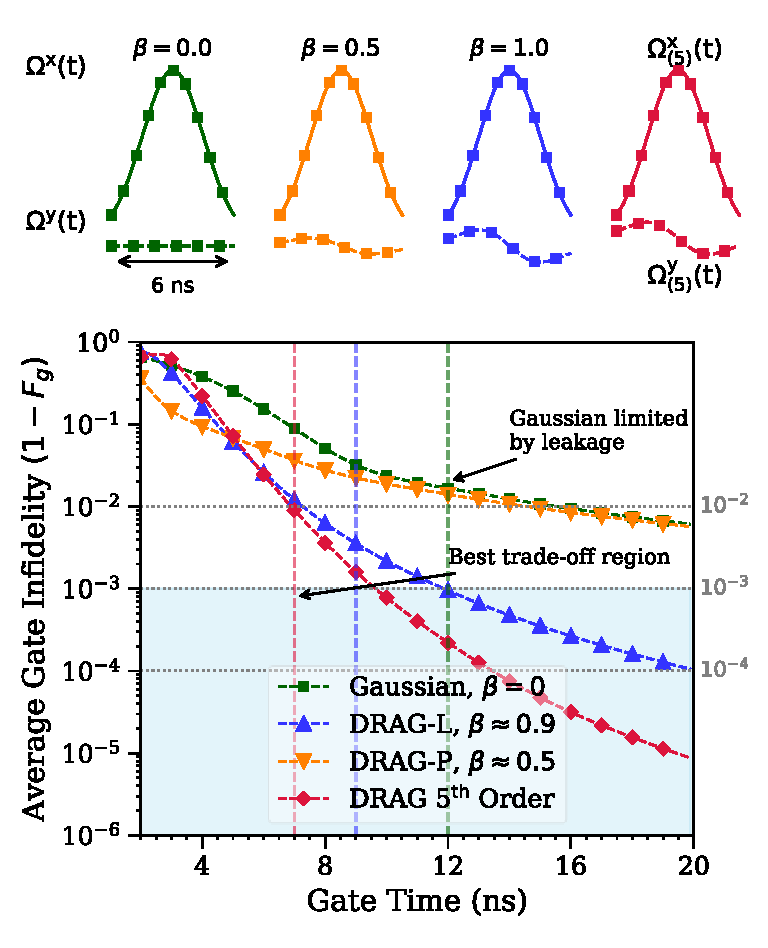
\includegraphics[width=0.8\linewidth]
    {gauss_envelopes.pdf}
    \vspace{-0.5cm}
    \caption{Pulse envelopes $\Omega^x(t)$ and $\Omega^y(t)$ for different DRAG parameters $\beta$, with $\beta=0$ corresponding to a Gaussian pulse, $\beta=0.5$ to the DRAG-P scheme (phase correction), $\beta=0.9$ to the DRAG-L scheme (leakage suppression), and the 5th-order DRAG correction \cite{ref3}. (Bottom) Average gate infidelity $(1-\mathcal{F})$ versus gate time (\(t_g\)), showing leakage-limited performance of the Gaussian and improved fidelity with DRAG schemes in the best trade-off region.}
    \label{fig1}
\end{figure}

\begin{figure}[h!]
    \centering
    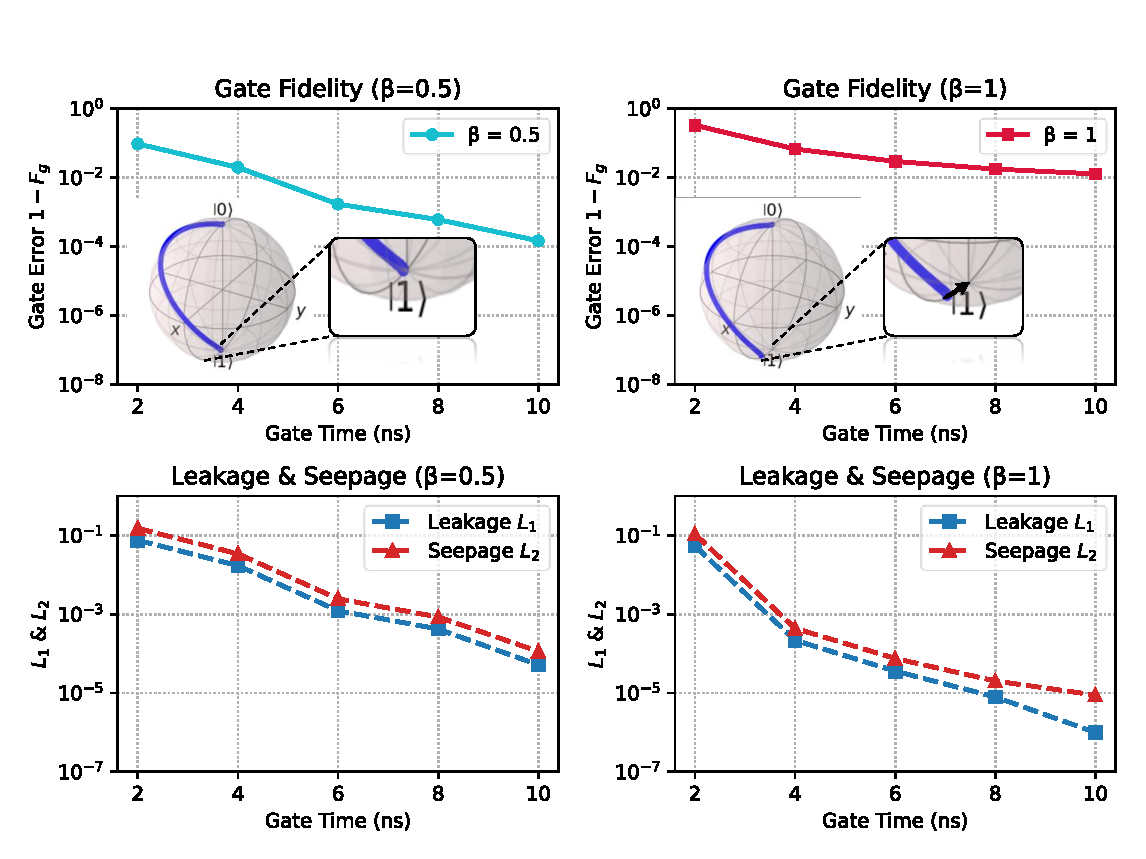
\includegraphics[width=1\linewidth]{fidelity_leakage_seepage.pdf}
    \caption{Gate performance for Gaussian DRAG pulses with $\beta=0.5$ (left) and $\beta=1.0$ (right). 
(Top) Gate fidelity versus gate time, with Bloch sphere trajectories showing qubit evolution. 
The $\beta=0.5$ case (DRAG-P) provides phase correction with limited leakage suppression, while $\beta=1.0$ (DRAG-L) yields stronger leakage suppression.  
(Bottom) Leakage $\mathcal{L}_1$ and seepage $\mathcal{L}_2$ \cite{ref4} as functions of gate time, both decreasing with longer gates, with $\beta=1.0$ giving superior suppression compared to $\beta=0.5$.}
    \label{fig2}
\end{figure}

\begin{figure*}[t]  % The * makes it span both columns
    \centering
    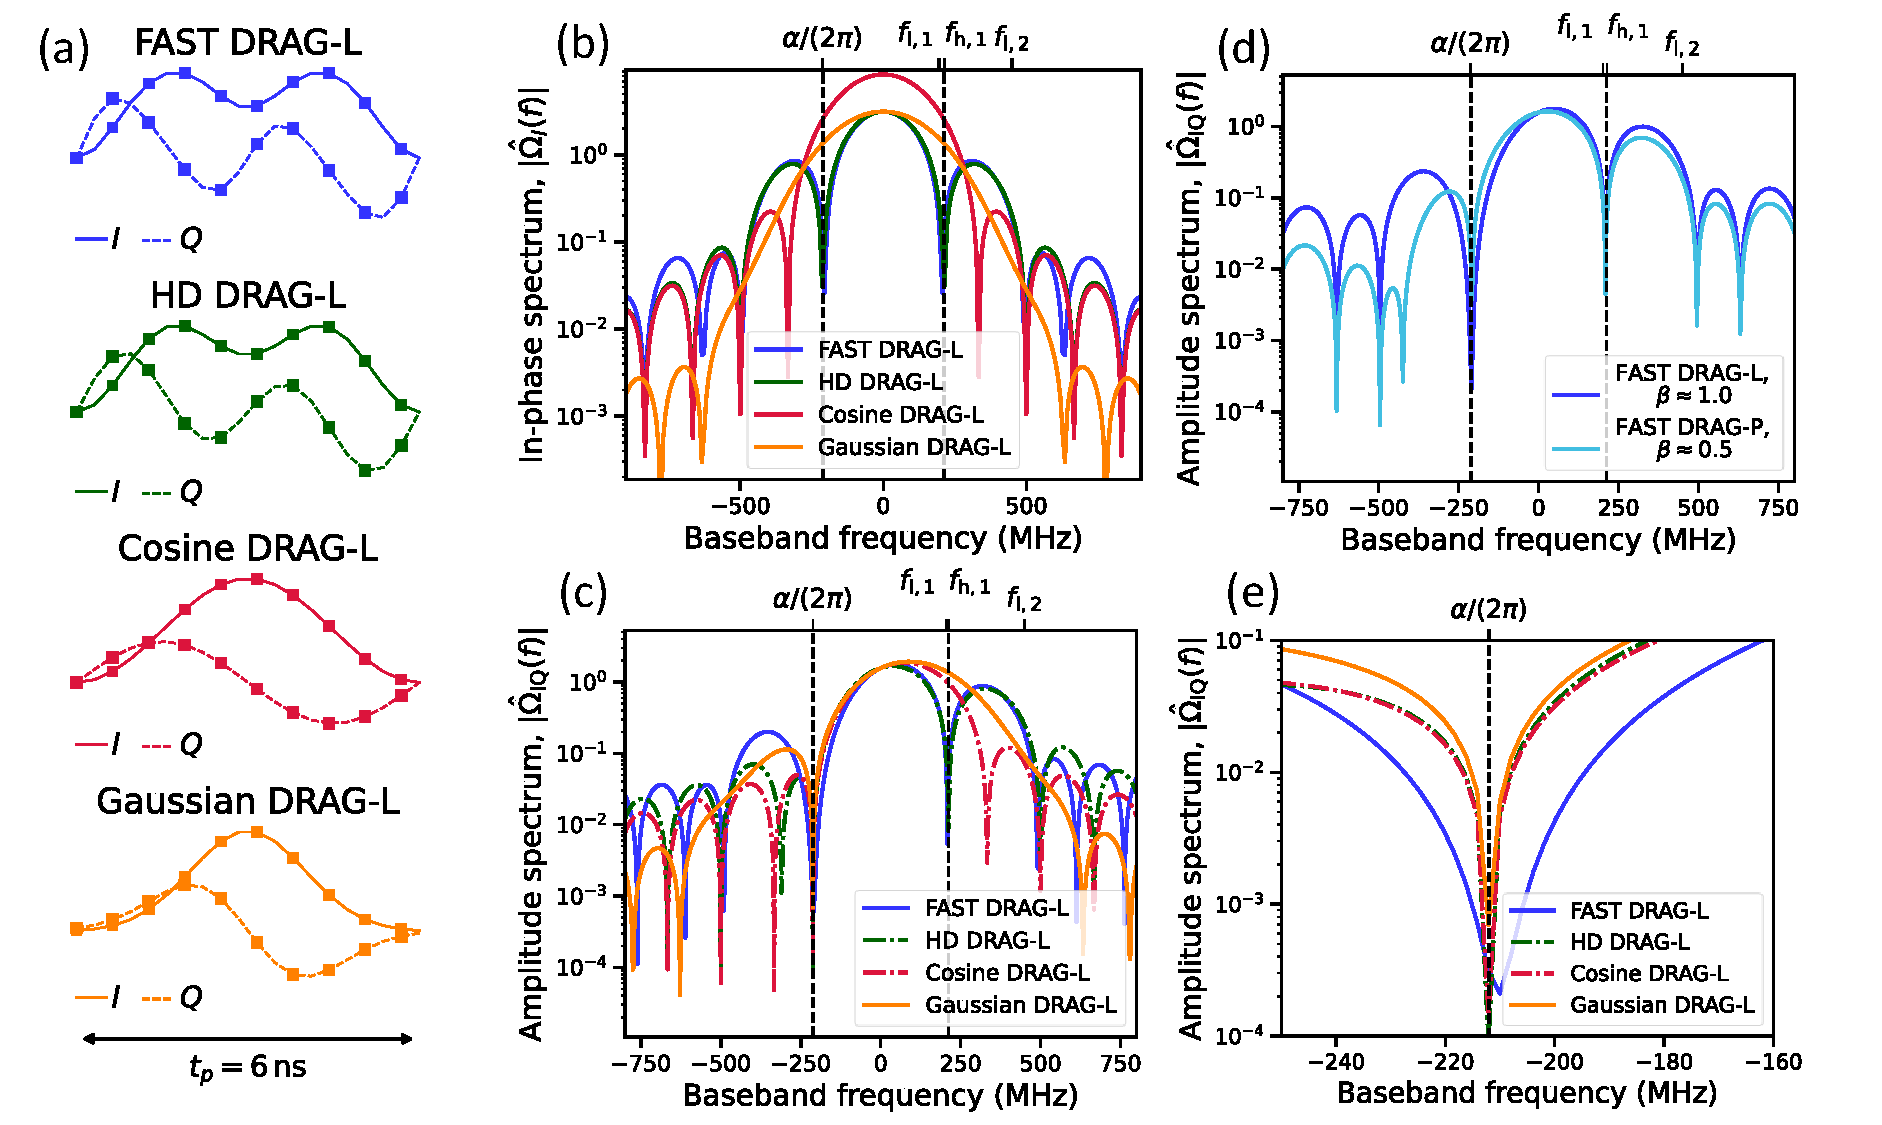
\includegraphics[width=0.9\textwidth]{leakage_spectrum.pdf}
    \caption{(a) Envelopes of the in-phase (\textit{I}, solid) and quadrature (\textit{Q}, dashed) components for two variants FAST DRAG-L (dark blue) and HD DRAG-L (darkgreen) with $\beta \approx 1.0$, both with same basis cosine function. The third one for conventional cosine DRAG pulse (red) with forth-one of extended gaussian DRAG pulse (dark orange) (b) Amplitude spectrum $\lvert \hat\Omega_I(f) \rvert$ of the in-phase envelope $I(t)$ for the same pulses. (c)  Amplitude spectrum $\lvert \hat\Omega_{IQ}(f) \rvert$ of the complex IQ envelope  $\Omega_{IQ}(t)$ for the same pulses, using DRAG to suppress the spectrum at the  qubit anharmonicity $\alpha / (2\pi)$ (dashed line). (d) Leakage spectrum for the FAST DRAG-L and FAST DRAG-P variants shown maximum suppression by DRAG-L. (d) Zoomed-in plot of figure~3(c) shows the suppression comparisons of the above pulses.}   
    \label{fig:wide-figure}
\end{figure*}
\noindent
 Here we are applying an additional pulse in the y-quadrature for mitigating the leakage, popularly known as Derivative Removal Adiabatic Gate (DRAG) - pulse, which is ideally the derivative of in-phase pulse \(\Omega^y(t) = -\beta\dot\Omega^x(t)/\alpha\).
In Fig.~\ref{fig1}, we illustrate the effect of four-different Gaussian DRAG \cite{ref3} schemes on fidelity under time-dependent detuning \(\delta(t)\), typically implemented via a flux line. Gate performance was quantified through average gate infidelity across multiple initial states. The colored vertical lines mark the gate durations required to reach an error of $\sim 10^{-2}$ for corresponding color pulse schemes. Notably, the 5th-order DRAG and DRAG-L pulses both achieve $99\%$ fidelity at $\sim 7\,\mathrm{ns}$, whereas Gaussian and DRAG-P pulses require about $12\,\mathrm{ns}$ to reach the same fidelity. Although higher-order DRAG and DRAG-L further suppress errors down to $10^{-4}$, decoherence at longer gate times limits their advantage, yielding an optimal operating window (sweet point) between $7$ and $12\,\mathrm{ns}$.
\newline \newline 
\noindent
In Fig.\ref{fig2}, we compare the gate infidelity $(1-\mathcal{F})$ together with leakage $(\mathcal{L}_1)$, of how much population leaked from the computational space and seepage $(\mathcal{L}_2)$, of how much population comes back to the computational states. \cite{ref4} as functions of gate time $(t_g)$ for DRAG-P ($\beta = 0.5$) and DRAG-L ($\beta = 1.0$). For DRAG-P, the gate error decreases below $10^{-4}$ at final gate times, whereas for DRAG-L it saturates around $10^{-2}$. Both schemes effectively suppress leakage: DRAG-P keeps it below $10^{-4}$, while DRAG-L pushes it further below $10^{-6}$. This comparison shows that fidelity is more sensitive to phase error accumulation evident from the Bloch sphere trajectories in the fidelity plots which is being corrected with time-dependent detuning in Fig.\ref{fig1} than to leakage. Phase error generally being corrected both in the start and in the end of the pulse applied by applying Virtual-Z \cite{ref5} gate at the software level.  
\newline \newline \noindent
Finally, we implemented Fourier Ansatz Spectrum Tuning (FAST DRAG) and Higher-Derivative DRAG (HD DRAG) \cite{ref1}, both of which enhance spectral control and suppress leakage at the anharmonic frequency. To implement fast, low-leakage single qubit gates, we combine the FAST method with DRAG by using FAST to shape the in-phase envelope of the control pulse and applying DRAG to obtain the quadrature component to combine FAST DRAG illustrated in Fig~3(a). It's advantage over others include stronger and wider spectral suppression over the traditional raised cosine illustrated in Fig.~3(e). To achieve this, we apply the FAST method to suppress the spectrum of in-phase envelope across the frequency interval \(\alpha/2\pi \in [f_{l,ef}, f_{h, ef}] = [f_{l1}, f_{h,1}]\) and use DRAG-L with \(\beta \approx1\) to further suppress the fourier transform \(\hat\Omega_{IQ}(f)\) of the complex envelope. Along with this it also reduces the bandwidth of the control pulse or lower the peak amplitude by using a second frequency interval \([f_{l2},f_{h,2}]\) to reduce the spectral energy above a given cuttoff frequency \(f_c = f_{l2}\). Both the FAST DRAG-L and FAST DRAG-P varients, the pulse and spectra are illustrated in Fig.~3(a) and Fig.~3(d). HD DRAG minimizes the in-phase envelope spectrum around the qubit anharmonicity while additionally using DRAG to further suppressing leakage. Here we consider derivative upto 2nd order in \(\Omega_I(t)\) envelope and till 3rd order in \(\Omega_Q(t)\). 
\newline\newline \noindent
Despite being similar, HD DRAG has less parameters to calibrate than FAST DRAG and can suppress multiple leakage transition by introducing higher derivatives. Although, HD DRAG does not allow straightforward control over the pulse bandwidth, the average power, or the exact strength and width of the spectral suppression unlike FAST DRAG, which offers more flexibility for the pulse design. Hence, we foresee that the flexibility of FAST DRAG is beneficial especially in scenarios with multiple leakage transitions.
\newline\newline\noindent
\textit{The Conclusion ---}
This work highlights various techniques for improving the overall fidelity of single-qubit gates, primarily by suppressing leakage errors. We have discussed several control schemes, including DRAG, fifth-order DRAG, FAST DRAG, and the HD DRAG method. Among these, the FAST DRAG scheme emerges as the most robust and flexible, with the added advantage of being easily calibratable at the hardware level.
Additionally, we examined the sensitivity of average gate fidelity to phase errors. These errors can be effectively mitigated using software-level corrections such as the virtual-Z gate, applied before and after the control pulse. Alternatively, phase accumulation can be minimized through time-dependent detuning, which dynamically adjusts the qubit energy levels during gate operation.  
\newline \newline \noindent
\textit{Future-aspects --} We can develop a mechanism to operate on the intermediate states of a multi-qubit system by designing pulses that first suppress spectral components at the primary anharmonicity, followed by suppression at the secondary anharmonicity.
\newline \newline 

\vspace{30cm}
% \begin{minipage}[t]{0.48\textwidth}
\begin{thebibliography}{99}
\bibitem{ref1} 
E. Hyyppä, A. Vepsäläinen, M. Papič, C. F. Chan, S. Inel, A. Landra, W. Liu, J. Luus, F. Marxer, C. Ockeloen-Korppi, S. Orbell, B. Tarasinski, and J. Heinsoo, 
"Reducing leakage of single-qubit gates for superconducting quantum processors using analytical control pulse envelopes", 
\textit{PRX Quantum}, vol. 5, no. 3, pp. 030353, 2024.

\bibitem{ref2}
J. Koch, T. M. Yu, J. Gambetta, A. A. Houck, D. I. Schuster, J. Majer, A. Blais, M. H. Devoret, S. M. Girvin, and R. J. Schoelkopf, 
"Charge-insensitive qubit design derived from the Cooper pair box", 
\textit{Physical Review A}, vol. 76, no. 4, pp. 042319, October 2007.

\bibitem{ref3}
F. Motzoi, J. M. Gambetta, P. Rebentrost, and F. K. Wilhelm, 
"Simple pulses for elimination of leakage in weakly nonlinear qubits", 
\textit{Physical Review Letters}, vol. 103, no. 11, pp. 110501, September 2009.

\bibitem{ref4}
C.J. Wood and J.M. Gambetta,
“Quantification and Characterization of Leakage Errors”,
\textit{Physical Review A}, vol. 97, no. 3, pp. 032306, March 2018.

\bibitem{ref5}
A. Vezvaee, V. Tripathi, D. Kowsari, E. Levenson‑Falk, and D. A. Lidar,  
“Virtual Z gates and symmetric gate compilation”,  
\textit{PRX Quantum}, vol. 6, no. 2, pp. 020348, June 2025.

\bibitem{ref6} 
F. Motzoi, J. M. Gambetta, P. Rebentrost, and F. K. Wilhelm, 
"Simple pulses for elimination of leakage in weakly nonlinear qubits", 
\textit{Physical Review Letters}, vol. 103, no. 11, pp. 110501, September 2009.
\end{thebibliography}
% \end{minipage}

\end{document}
